\documentclass{sig-alternate}
\usepackage[utf8]{inputenc}
\usepackage{listings}

\lstset{
language=Java,
basicstyle=\footnotesize,
showtabs=false, 
showspaces=false,
showstringspaces=false,
frame=single,
breaklines=true,
tabsize=2,
captionpos=b
}


\begin{document}

\conferenceinfo{MSR}{Mining Software Repositories '14}

\title{How to Calculate Code Coverage\\
Without Running the Tests?\\
An Heuristic Using Statical Code Analysis}

\numberofauthors{2}

\author{
\alignauthor
Mauricio Aniche\\
\affaddr{Institute of Mathematics and Statistics}\\
\affaddr{University of São Paulo}\\
\email{aniche@ime.usp.br}
\alignauthor
Marco Aurelio Gerosa\\
\affaddr{Institute of Mathematics and Statistics}\\
\affaddr{University of São Paulo}\\
\email{gerosa@ime.usp.br}
}

\maketitle
\begin{abstract}

bla bla bla bla bla bla bla bla bla bla bla bla bla bla bla bla bla bla bla bla bla bla bla bla
bla bla bla bla bla bla bla bla bla bla bla bla
bla bla bla bla bla bla bla bla bla bla bla bla
bla bla bla bla bla bla bla bla bla bla bla bla
bla bla bla bla bla bla bla bla bla bla bla bla
bla bla bla bla bla bla bla bla bla bla bla bla


\end{abstract}

\section{Introduction}

One advantage of studies that make use of mining software repository techniques
is that it can be done on a large quantity of projects and data. This enormous 
quantity of information allows researchers to validate a phenomenon with more
property.

Researchers can extract data from many different sources, such as issue trackers,
source code repositories, mailing lists, and so on. Most of them are text-based, which
means that the researcher should only find a way to extract and then process it. 
However, source code is tricky: some metrics need the code to be compiled first.

Compiling code is a complicated task. Each project has its own build process and
required libraries. It is common that many of them are not available at the time the
researcher has the source code.

An example of code metric that usually requires compiled code is code coverage. 
The metric calculates the percentage of the production code that is covered by at least
one unit test. Popular tools, such as Emma\footnote{http://emma.sourceforge.net/} or
Cobertura\footnote{http://cobertura.github.io/cobertura/}, instrument the code, execute
the unit test suite, and then extract the information. As said before, when dealing
with many different repositories, compiling and executing unit tests may not be
an alternative.

% TODO: colocar aqui as secoes
To sort this problem out, we present an heuristic to calculate code coverage without
compiling or even running the unit tests. In Section X, we discuss bla bla bla,
bla bla bla bla bla bla bla bla bla bla bla bla bla bla bla bla bla bla ,
bla bla bla bla bla bla bla bla bla bla bla bla bla bla bla bla bla bla 
bla bla bla bla bla bla bla bla bla bla bla bla bla bla bla bla bla bla\cite{bowman:reasoning}.

% TODO: explicar um pouco dos findings



\section{Code Coverage}

Code coverage measures the quantity of production code that is being tested by
the test suite. When a unit test exercises a piece of code, developers say that the piece
of code is covered. The common output of the tools is a percentage, which is calculated
by the quantity of production code lines that are covered by at least one unit test divided by
the total number of production code lines.

There are many different ways to calculate code coverage. The tool can calculate the number
of lines (as mentioned before), the number of instructions, the number of conditions, and even
the number of executed branches.

As mentioned before, Emma and Cobertura are popular tools. 
They both use dynamic analysis to calculate the metric. They instrument the code, 
execute the unit test suite, and then discover which instructions were executed.
Besides taking a long time to calculate (as they need to execute the entire test suite),
they require compiled code.

\section{The Heuristic}

% TODO: ref para mccabe
As we wanted to avoid dynamic analysis, the only option was to apply statical analysis to
the source code. The first step was to estimate the maximum number of tests that a class
(or a method) needed. To do that, we decided to use McCabe's cyclomatic complexity \cite{mccabe}.
McCabe's number basically shows the different number of execution paths per method. The listing
\ref{simple-code} below exemplifies it. In that case, McCabe's number would be 2.
As we are calculating code coverage in class method, we calculate the class' cyclomatic complexity
by summing up McCabe's number of all methods.

\lstset{caption={McCabe's number to this method is 2.},
label={simple-code}}
\begin{lstlisting}
public void doSomething(int a) {
	int total = 0;
	if(a>10) total += 1;
	return total;
}
\end{lstlisting}

The next step was to count the number of unit tests that invoke a specific production method. To do that,
in a statically, we count all the invocations that happens in the unit tests. As an example, in Listing
\ref{unit-test}, we consider the invocation to \textit{calculateTaxes()} as a unit test to it.
We then repeat this procedure to all unit tests.

\lstset{caption={An example of a unit test},
label={unit-test}}
\begin{lstlisting}
class InvoiceTest {
	@Test
	public void shouldCalculateTaxes() {
		Invoice inv = new Invoice("Customer", 5000.0);

		double tax = inv.calculateTaxes();
		double taxAgain = inv.calculateTaxes();
		
		assertEquals(5000 * 0.06, tax);
	}
}
\end{lstlisting}

We then calculate the ratio between the number of tests and 
McCabe's number. In the Figure \ref{fig:formula}, we show the formula.
Suppose that the class \textit{Invoice} has McCabe's number equals to 10, and there are 6 unit tests
that invoke methods that belong to it.  
In this case, \textbf{6 / 10 = 0.6}, which means \textbf{60\%} of code coverage.


	\begin{figure}[h!H]
	  \centering
	  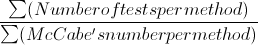
\includegraphics[scale=0.6]{imgs/formula.png}
	  \caption{Formula used to calculate code coverage in our heuristic}
	  \label{fig:formula}
	\end{figure}


There are a few exception cases that are worth mentioning. 
As we are
interested in the number of distinct unit tests per production method, even if a test invokes the same method twice, it
counts as one. In the example above, \textit{calculateTaxes()} is invoked twice, but we only mark that it is being
tested by \textit{shouldCalculateTaxes()}.

\section{Experiment Design}

To validate the heuristic, we decided to compare the code coverage calculated by it with the ones 
calculated by a dynamic analysis tool. We chose Emma as we had a previous experience with it. We
had 3 projects as subjects, all of them developed by the same company, in Java. Two of them are
web applications and one of them is a console application. In Table \ref{tab:projects}, we describe
the size of each one.

\begin{table}[h!]
\centering
\caption{Quantity of classes and methods per project}
\begin{tabular}{ | l | r | r | r | }
\hline
& Classes & Production Methods & Unit Tests\\ 
\hline
Gnarus & 769 & 1823 & 826\\ 
MetricMiner & 225 & 1009 & 341\\ 
Tubaina & 261 & 372 & 298\\ 

\hline
\end{tabular}
\label{tab:projects}
\end{table}

With both code coverage numbers (Emma's and ours), we then compared both to see how different
they were. In Section below, we present the results found.

\section{Findings}

To do the analysis, we decided to use the number calculated by our heuristic minus the
number calculated by Emma. It means that every time we find a zero, it meant that both numbers
were equal, and the heuristic was perfect. A negative number indicates that the heuristic calculated
a smaller number than the real; a positive number indicates that the heuristic calculated a higher
number.

In Figure \ref{fig:metricminer}, we show the histogram of the difference between Emma and our approach to
the MetricMiner project.
In the X axis, we have the difference (from -1 to 1), and in the Y axis, we have the frequence of that difference.
By looking to this Figure, one can notice that most of the data are between -0.2 and 0.2. 
The median of the distribution is 0, and the mean is 0.1149. The first quartile is 0, and the
third quartile is 0.2414.

\begin{figure}[h!H]
  \centering
  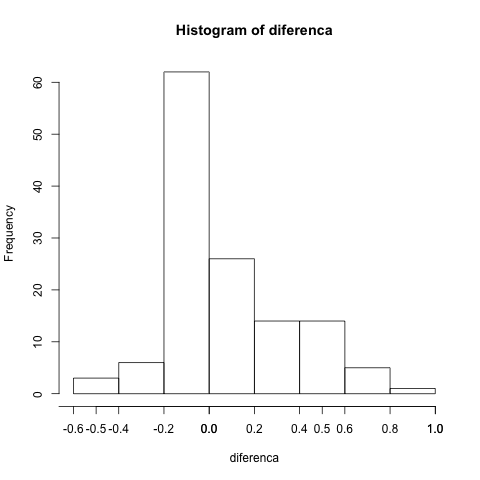
\includegraphics[scale=0.5]{imgs/metricminer-histograma.png}
  \caption{Our approach compared to Emma's in the MetricMiner}
  \label{fig:metricminer}
\end{figure}

In Figure \ref{fig:tubaina}, from Tubaina project, the data is between
-1 and 0. The median is 0, and the mean is 0.0790. The first quartile is
0, and the third quartile is 0.1667.

\begin{figure}[h!H]
  \centering
  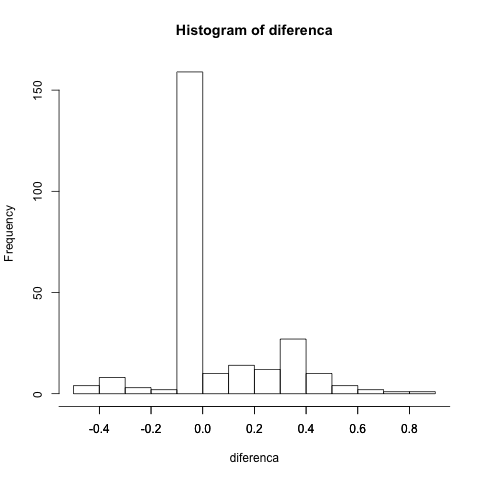
\includegraphics[scale=0.5]{imgs/tubaina-histograma.png}
  \caption{Our approach compared to Emma's in the Tubaina}
  \label{fig:tubaina}
\end{figure}


In Figure \ref{fig:gnarus}, from Gnarus project, we can see that most of data
are between -2 and 0. The median is 0, the mean is -0.0152. The first quartile
is -0.7273, and the third quartile is 0.

\begin{figure}[h!H]
  \centering
  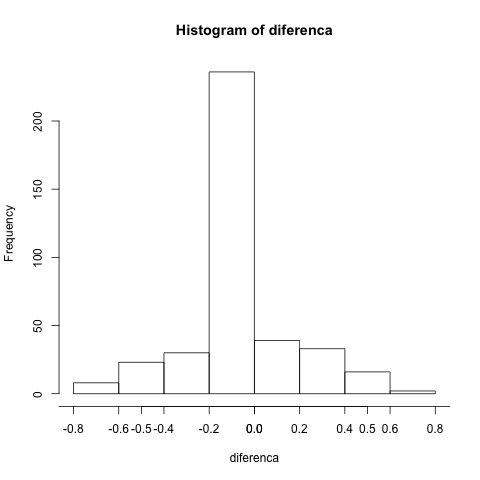
\includegraphics[scale=0.5]{imgs/gnarus-histograma.png}
  \caption{Our approach compared to Emma's in the Gnarus}
  \label{fig:gnarus}
\end{figure}

\section{Discussion}

Based on the numbers presented in the section above, we believe that the heuristic
is acceptable. As the maximum mean error was 0.1149 found in these 3 projects, which means 11\%, 
we do not think that it will be a problem when using it in large software repositories.

% olhar as classes que deram muita diferenca e entender o pq, pra falar os problemas

As Emma needs to execute the tests, and they may take a long time to execute, we also argue
that our approach is faster.

\section{Threats to Validity}

o algoritmo pode ter problemas

os projetos foram desenvolvidos pelos devs de uma soh empresa e eles tem a maneira de escrever
os testes, entao sao 3 aplicacoes parecidas em termos de arquitetura.

\section{Related Work}

%Yes, check Q1.2 (page 31) and Assertions-McCabe ratio (page 33) in my thesis: 
% http://swerl.tudelft.nl/twiki/pub/Main/PastAndCurrentMScProjects/Thesis_DimitriosAthanasiou.pdf

% tiago miguel aureliano

% http://www.cse.cuhk.edu.hk/~lyu/paper_pdf/paper20.pdf

% http://testingeducation.org/BBST/foundations/Marick_coverage.pdf

% http://digitalcommons.unl.edu/cgi/viewcontent.cgi?article=1128&context=cseconfwork

% http://ieeexplore.ieee.org/xpls/abs_all.jsp?arnumber=497650

% http://citeseerx.ist.psu.edu/viewdoc/download?doi=10.1.1.46.4263&rep=rep1&type=pdf

% http://dl.acm.org/citation.cfm?id=961347

% http://ieeexplore.ieee.org/xpls/abs_all.jsp?arnumber=902502

% http://scholarsarchive.library.oregonstate.edu/xmlui/bitstream/handle/1957/10219/Joseph_Lawrance.pdf?sequence=1

\section{Conclusion and Future Work}

rodar em mais projetos

melhorar a ferramenta que ainda tem problemas

\section{Acknowledgments}

bla bla

\bibliographystyle{abbrv}
\bibliography{sigproc}

\end{document}
